%\cia
\subsection{Drift chamber inefficiencies}
\label{sec:dc_ineff}
The Drift Chambers present inefficiencies which must be taken into account by the
the MonteCarlo simulation for a correct acceptance calculation.
As the DC is repaired or fails with time, each
experiment has a different drift chamber status. Some systems (for example HV) might 
fail during the experiment. 
 
What follows is the description of the calculation of a global DC efficiency
to exploit at once the DC
inefficiency and theirs time dependency.

Each CLAS sector has the same drift chamber configuration, shown in 
Table \ref{tab:layers}, which consists of three separate regions containing a 
total of 34 layers of sense wires. Region 1 has four layers, region 2 and 3 have
six layers each.  
\vspace{1cm}
\begin{table}[h]
 \begin{center}
  \begin{tabular}{| c | c c c c c c c c c c c c |}
   \hline
   Layer    & 1 & 2 & 3 & 4 & 5 & 6 & 7 & 8 & 9 & 10 & 11 & 12 \\
   \hline
   Region 1 & 130 & 130 & 130 & 130 &   0 &   0 & 142 & 142 & 142 & 126 & 121 & 120 \\
   Region 2 & 184 & 185 & 186 & 187 & 188 & 189 & 189 & 189 & 190 & 191 & 192 & 192 \\
   Region 3 & 192 & 192 & 192 & 192 & 192 & 192 & 192 & 192 & 192 & 192 & 192 & 192 \\
   \hline
  \end{tabular}  
  
  \caption[ Number of wires in each layer]
          { Number of wires in each layer. Region 1 has only 4 layers, so layers 5 and 6 are phantom.}
  \label{tab:layers}
 \end{center}
\end{table} \\
\F{fig:dc_occupancy} shows the occupancy of the drift chamber in sector 6 for the e1-6 experiment.

There are three wires pathologies:
\begin{itemize}
\item {\em holes}: there are nearly no counts in layers 34,35,36 near wire number $ 150$. 
                   This is an example of a {\em hole}. During tracking, a hole could affect track reconstruction 
		   because a minimum number of 
                   wires are required to define a track.

\item{\em hot} wires:  Wires that count significantly more than neighboring ones are ``hot''. Track reconstruction is basically undisturbed by 
                       those\footnote {This is an empirical statement.}.

\item{\em warm} wires: wires that count less than neighboring ones but not {\it substantially less}.
                       For example, a wire can count an average of $70\%$ relative to its neighbours. 
		       		      		       
\end{itemize}




\begin{figure}[h]
 \begin{center}
 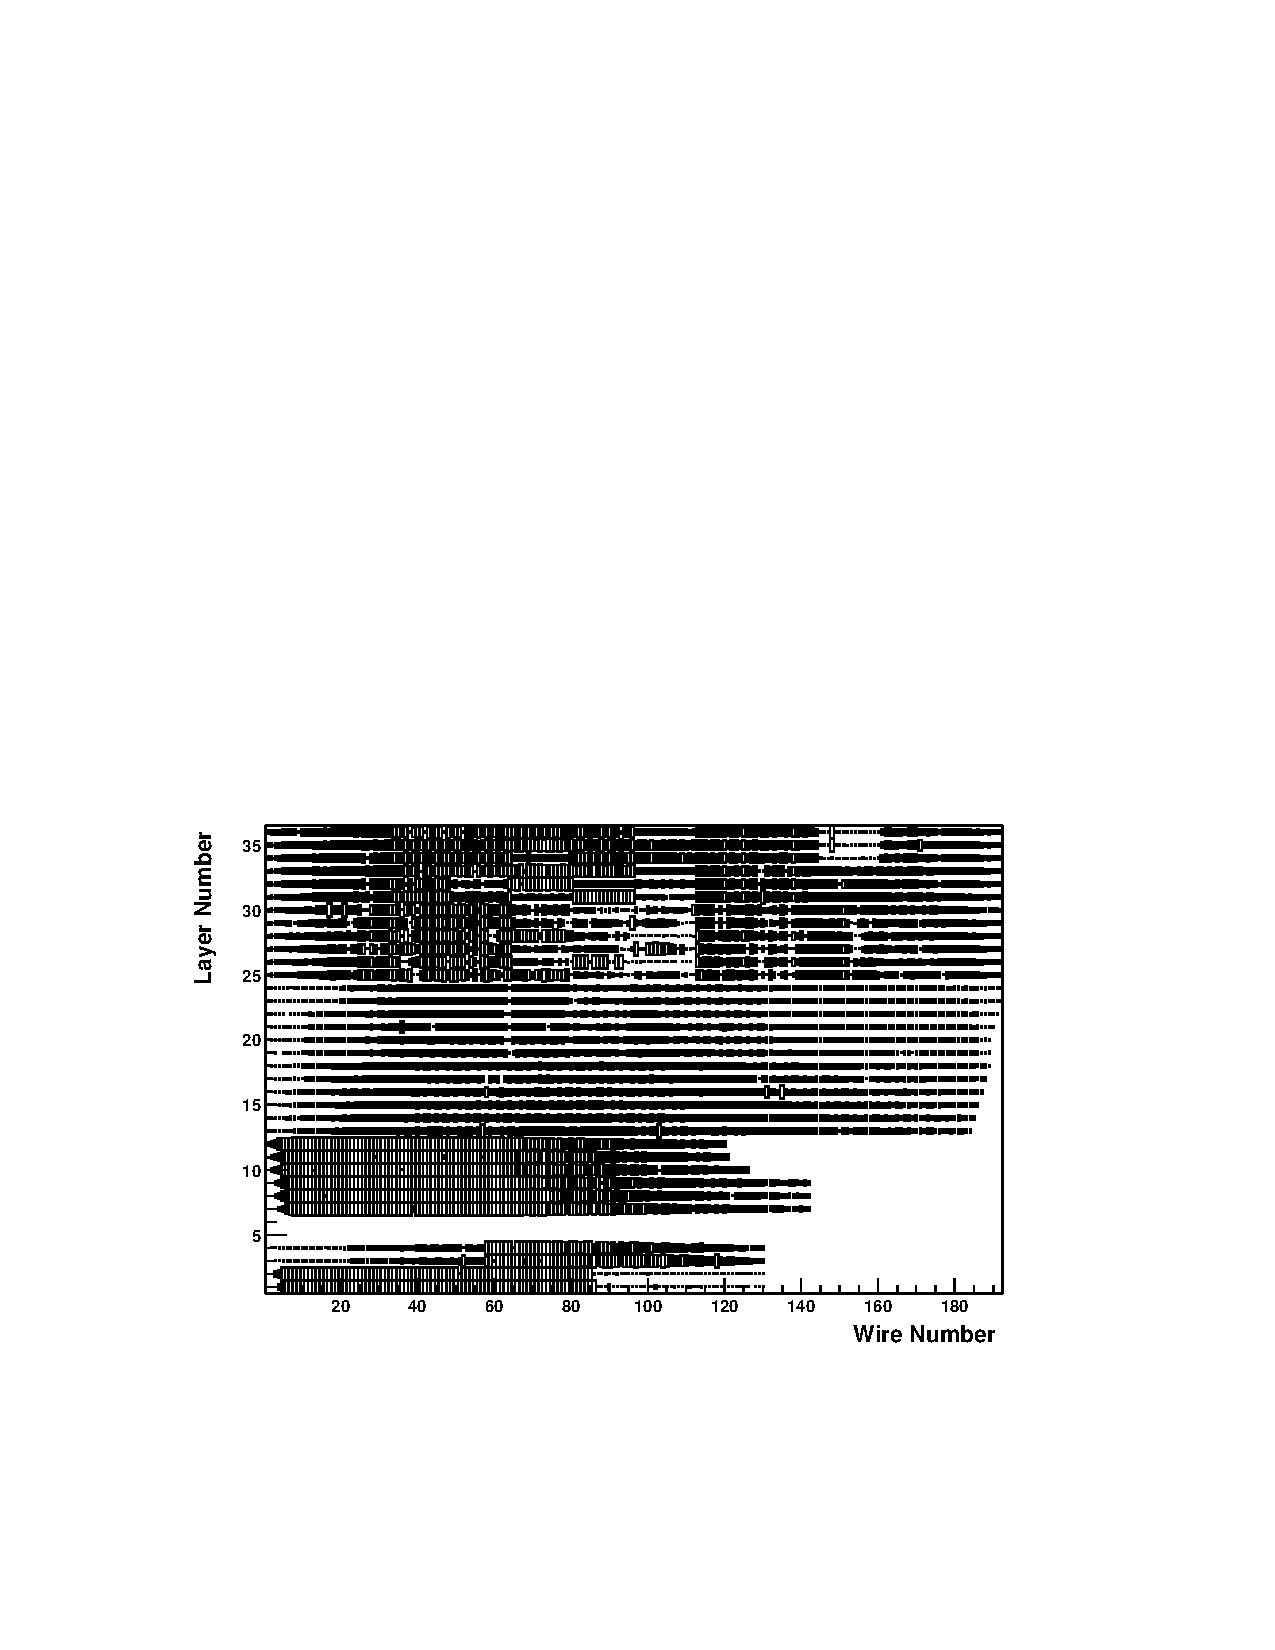
\includegraphics[width = 15cm, bb=40 150 580 420]{acceptance/img/sector6_occupancy} 
  \caption[Drift chamber occupancy distribution for sector 6]
          { Drift chamber occupancy distribution for sector 6. A hole is visible in 
	             layers 34-35-36 near wire number $ 150$.}
 \label{fig:dc_occupancy}
 \end{center}
\end{figure} 

Some warm wires could be correlated. For example they could be attached to the same (defective) 
ADB board\footnote{An {\bf A}mplifier {\bf D}iscriminator {\bf B}oard 
is a power supply unit. With a $60 Hz$ varying gain of threshold it might give a correlated efficiency.}, 
so that all wires in that board have {\it the same efficiency at the same time}.
Correlated wires affect tracking in that a group of wires might miss at the same instant, preventing the creation of a track segment.


In order to calculate the efficiency of a wire, the whole e1-6 period has been considered. If a wire has
 $50\%$ efficiency it could mean that
\begin{itemize}
\item it was efficient only half of the time, i.e. the chance of give a signal is $50\%$
\item the wire was alive for half the experiment and dead for the other half.
\end{itemize} 
so that the time dependancy problem of the DC has been been solved. 

For each  $w(i,S)$ of the $36,000$ wires, with $i$ being the wire index and $S$ its sector,
 a sample of $18$ wires has been considered:  its next neighbors in the same 
sector $w(i-1, S)$ and $w(i+1, S)$ and
the corresponding wires in all the other sectors $w(i, S')$, $w(i-1, S')$, $w(i+1, S')$.
Table \ref{tab:wire_sample} shows one example of such a sample.

\begin{table}[h]
 \begin{center}
  \begin{tabular}{ c c c c c c c }
   Layer & Sector 1 & Sector 2 & Sector 3 & Sector 4 & Sector 5 & Sector 6 \\
   $i_o$      & 670080 & 674517 & 681877 & 678828 & 676214 &   2207 \\
   $i_o - 1 $ & 736412 & 734450 & 738558 & 746698 & 739865 &   5281 \\
   $i_o + 1 $ & 678419 & 665103 & 685710 & 105299 & 410887 & 677456 \\
  \end{tabular}
 \caption[Example of 18 wires sample from real CLAS data]
         { Example of 18 wires sample from real CLAS data. For each of the 36,000 wires a similar sample is taken.}
 \label{tab:wire_sample}
 \end{center}
\end{table}

For each wire $w_J$ in the above sample, with $J=1...18$, 
the variable $buddies$ represents the number of wires in the same sample whose occupancy is within $8\%$ of $w_J$,
as illustrated in \F{fig:buddies}.
\begin{figure}[h]
 \begin{center}
 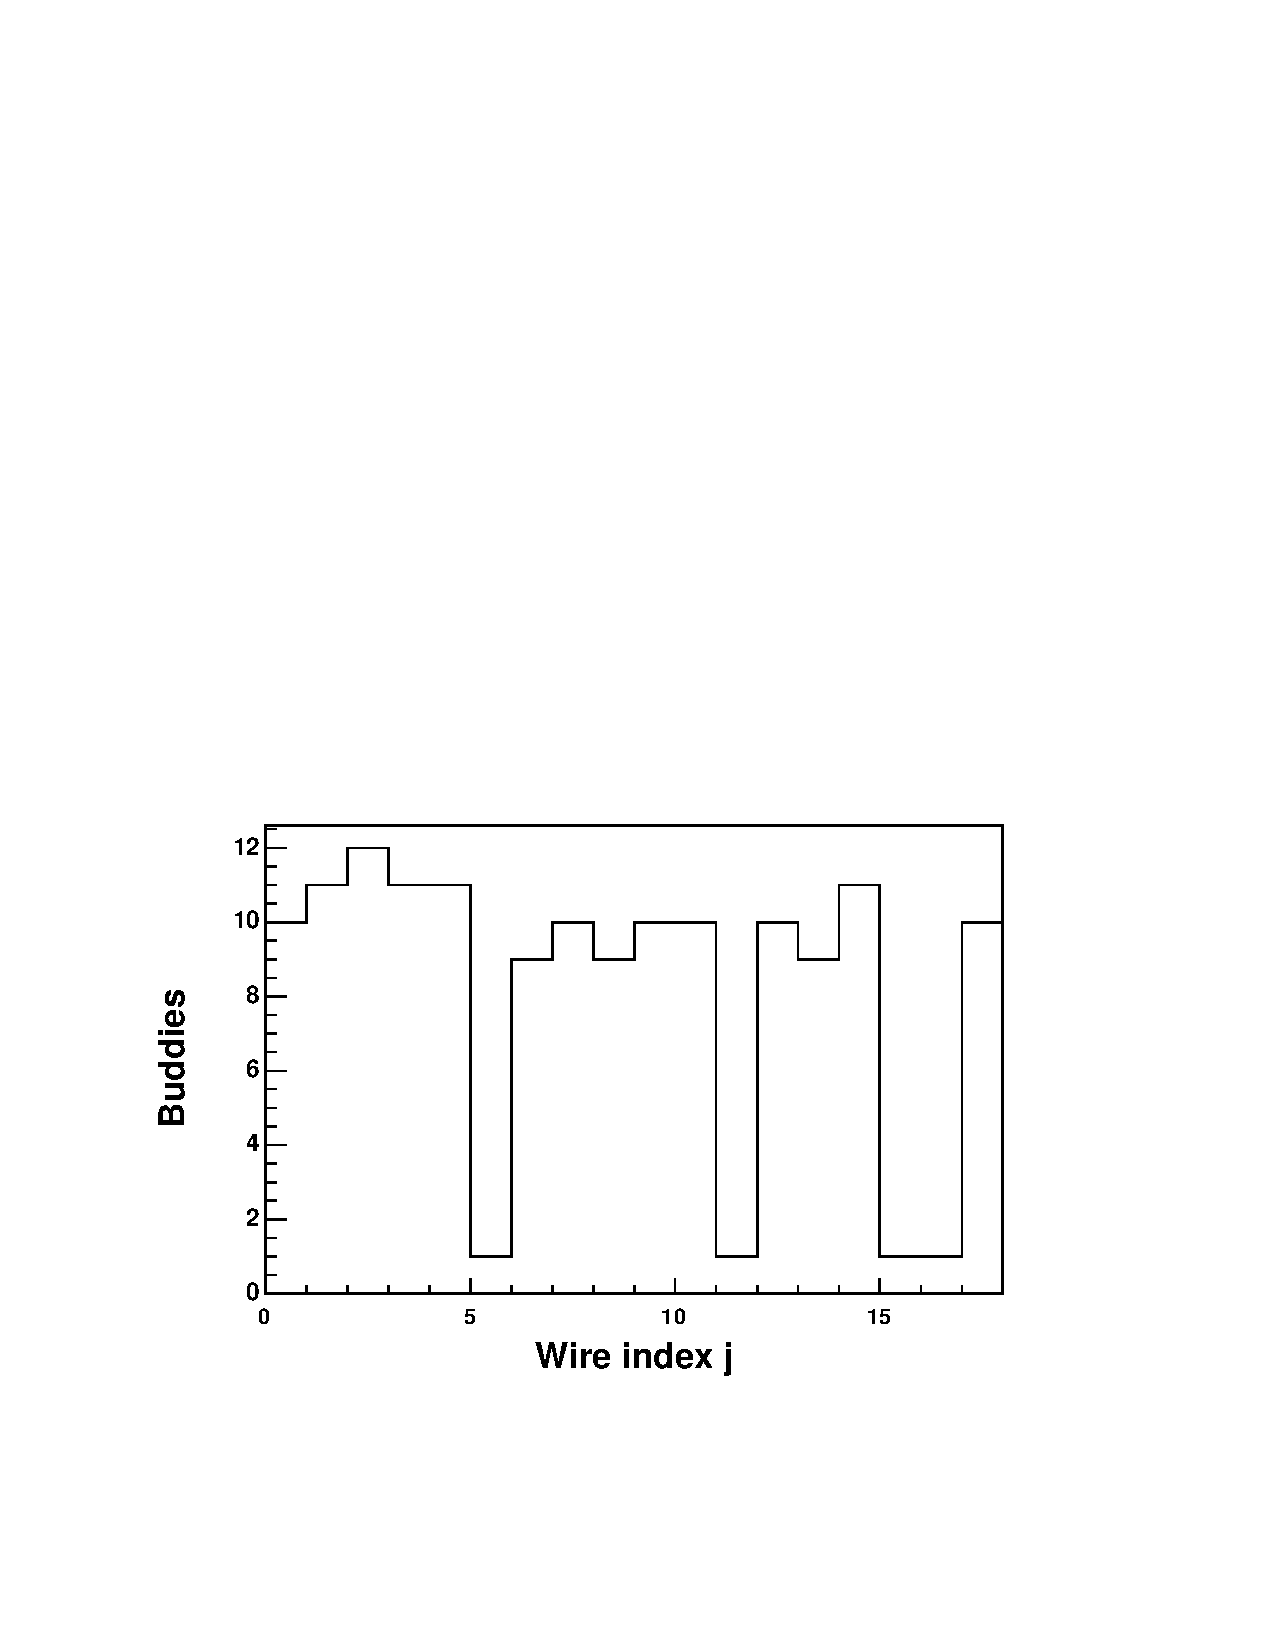
\includegraphics[width = 13cm, bb=0 120 580 420]{acceptance/img/buddies} 
  \caption[The next neighbor technique: the $buddies$ histogram]
          { The next neighbor technique: the $buddies$ histogram. Wire $3$ has the maximum number of $buddies$.}
 \label{fig:buddies}
 \end{center}
\end{figure} 

The sub-sample that maximizes $buddies$ is formed by good wires\footnote{Since 
usually there are $\sim 5,000$ defective wires among the $36,000$, the probability that 
they maximize $buddies$ is negligible. }. 
In this example wire 3 has 12 buddies.

The sub-sample is used to calculate the expectation value $A$ for the occupancy of $w(i,S)$. $A$ is the average
of the occupancy in the the sub-sample.
(in the example of table \ref{tab:wire_sample}
and \F{fig:buddies} $A = 695191$).

The efficiency of $w(i,S)$ is in this case
$$
 E = Occupancy/Expectation = 670080 / 695191 = 0.96387 
$$

An efficiency table was incorporated in clas database and the GSIM MonteCarlo output is processed so that
the simulated wire occupancy is a good representation of the real one \cite{bib:wires}. \F{fig:wires_comp} shows
the comparison of real and simulated efficiency for sector 5.


\begin{figure}[h]
 \begin{center}
 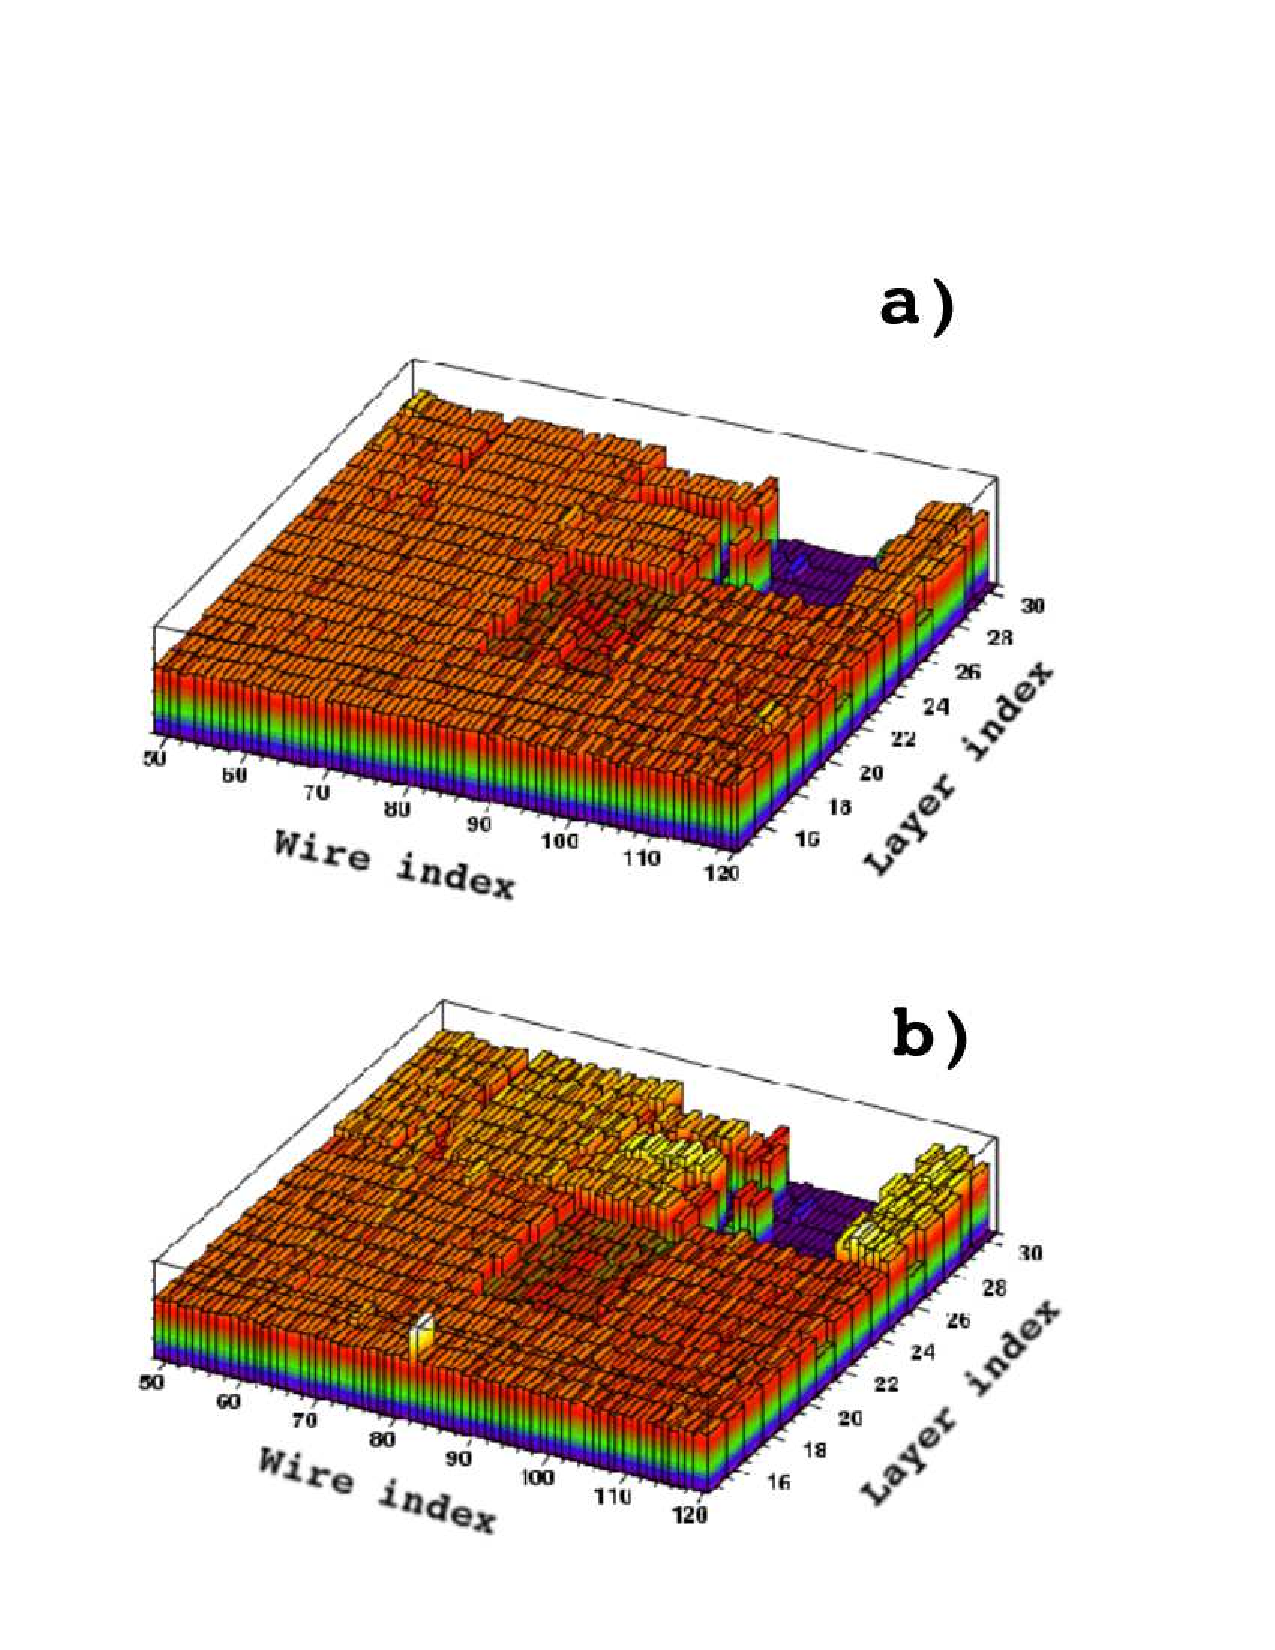
\includegraphics[width = 12cm, bb=0 0 700 720]{acceptance/img/wires_comp} 
 %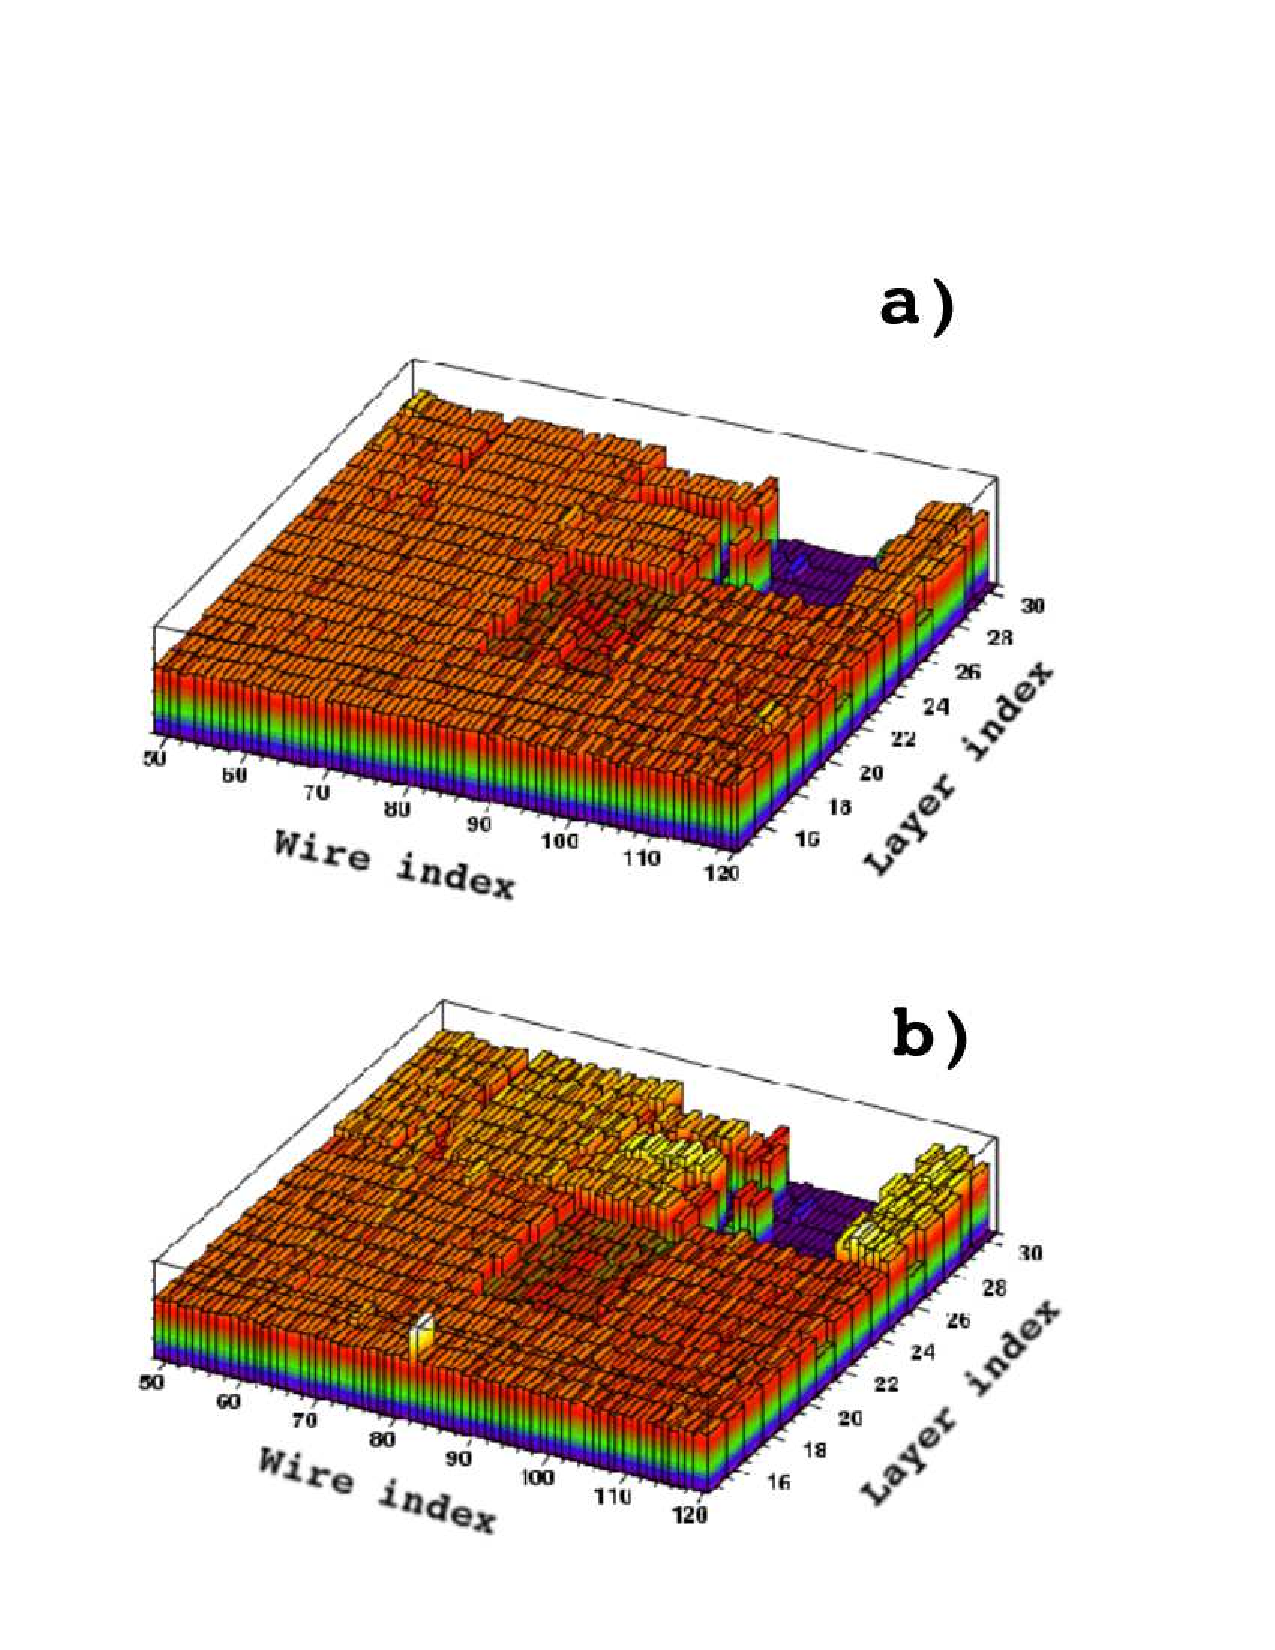
\includegraphics[width = 12cm]{acceptance/img/wires_comp}  
  \caption[Comparison between real and simulated efficiency.]
          { Comparison between real and simulated efficiency ($z-axis$) for sector 5. (a) simulation. (b) real data.
	             A hole at layers $26-28$ is visible. A Depleted region at layers $20-24$ is also visible. 
		     The hot wire ($i=80$) is not reproduced in the MonteCarlo because it does not affect the tracking.}
 \label{fig:wires_comp}
 \end{center}
\end{figure} 



























